
\documentclass[12pt]{article}
\usepackage{amsmath,amssymb,bm}
\usepackage{geometry}
\geometry{margin=1in}
\usepackage{tikz}
\usepackage{pgfplots}
\pgfplotsset{compat=1.18}
\usepackage{siunitx}
\sisetup{detect-all=true}

\title{Appendix L -- Standing and Modulated Electromagnetic Waves for Curvature Amplification (UBT)}
\date{}

\begin{document}
\maketitle

\section*{L.1 Motivation (UBT vs. GR/Maxwell)}
In standard General Relativity (GR) with classical electromagnetism (EM), standing or modulated EM waves do \emph{not} measurably curve spacetime in laboratory conditions because the EM stress--energy required is astronomically large.
In the Unified Biquaternion Theory (UBT), the complex time $\tau=t+i\psi$ introduces a slow, phase-sector degree of freedom. 
Small $\psi$-dependent deformations of the metric $g_{\mu\nu}\!\to g_{\mu\nu}+\delta g_{\mu\nu}(\psi)$ can \emph{interfere} with structured EM fields so that curated standing/modulated modes act as a lever on curvature.
Where $\psi\!=\!0$ (or averages to zero), UBT reduces to GR/Maxwell and remains compatible with existing experiments.

\section*{L.2 Field Model in a Cavity (Standing+Modulated)}
Consider an axisymmetric cavity supporting a single longitudinal component $U(\mathbf{r},t)$ obeying the curved-space Helmholtz equation (Appendix K).
A representative standing wave with slow amplitude modulation is
\begin{equation}
U(\mathbf{r},t)=U_0 \cos(kr)\cos(\omega t)\,\bigl[1+m\cos(\Omega t)\bigr],\qquad 0<m<1,\ \ \Omega\ll \omega,
\end{equation}
and a slow phase modulation $\phi(t)$ can be added as $\cos(\omega t+\phi(t))$.
The local (time-averaged over $2\pi/\omega$) EM energy density is, schematically,
\begin{equation}
\langle \mathcal{E}\rangle \propto \tfrac{1}{2}\epsilon_{\rm eff} \langle |E|^2\rangle + \tfrac{1}{2}\mu_{\rm eff} \langle |H|^2\rangle \;\propto\; U_0^2 \cos^2(kr)\,\Bigl(1+\tfrac{m^2}{2}\cos^2\Omega t\Bigr)+\cdots,
\end{equation}
which defines an effective stress--energy $T^{\mu\nu}_{\rm EM,eff}$ entering curvature in GR and, in UBT, couples also to $\psi$ through $\delta g(\psi)$.

\section*{L.3 Effective Curvature Lever in UBT}

\subsection*{L.3.1 Effective Electromagnetic Stress--Energy $T^{\mu\nu}_{\rm EM,eff}$ (UBT)}
In UBT the EM sector couples to the phase field $\psi$ so that the effective stress--energy sourcing curvature is
\begin{equation}
T^{\mu\nu}_{\rm EM,eff} \;=\;
\frac{1}{\mu_0}\!\left(F^{\mu\alpha}F^{\nu}{}_{\alpha} - \frac{1}{4}g^{\mu\nu}F_{\alpha\beta}F^{\alpha\beta}\right)
\;+\; \lambda_\psi\,\Psi^{\mu\nu}(\psi,F)\,,
\label{eq:Tem_eff}
\end{equation}
with a UBT correction tensor $\Psi^{\mu\nu}$ that vanishes when $\psi\!\to\!0$. A minimal gauge-invariant choice is
\begin{equation}
\Psi^{\mu\nu}(\psi,F) \;=\; \psi\,\Big(F^{\mu\alpha}F^{\nu}{}_{\alpha} - \frac{1}{4}g^{\mu\nu}F_{\alpha\beta}F^{\alpha\beta}\Big)
\;+\; \eta^{\mu\nu}\,\psi\,\frac{\tilde{F}_{\alpha\beta}F^{\alpha\beta}}{4}\,,
\end{equation}
where $\tilde{F}^{\alpha\beta}$ is the dual field tensor; the second term parametrizes parity-odd couplings if present.
The coupling $\lambda_\psi$ aggregates UBT constants and, in standing/modulated modes, is probed at the slow rate $\Omega \ll \omega$.

\subsection*{L.3.2 Linearized Metric Response $\Delta g_{\mu\nu}$}
In the weak-field limit, with $\bar{h}_{\mu\nu}=h_{\mu\nu}-\tfrac{1}{2}\eta_{\mu\nu}h$ in Lorenz gauge,
\begin{equation}
\square\,\bar{h}_{\mu\nu} \;=\; -\,\frac{16\pi G}{c^4}\,T^{\rm eff}_{\mu\nu}\,,
\qquad
h_{\mu\nu}\equiv \Delta g_{\mu\nu}\,.
\end{equation}
The retarded solution is
\begin{equation}
h_{\mu\nu}(t,\mathbf{x}) \;=\; -\,\frac{4G}{c^4}\int d^3x'\,
\frac{T^{\rm eff}_{\mu\nu}(t-\tfrac{|\mathbf{x}-\mathbf{x}'|}{c},\mathbf{x}')}{|\mathbf{x}-\mathbf{x}'|}\,.
\label{eq:retarded_h}
\end{equation}
For a cavity mode normalized over volume $V$, the mode-averaged fractional frequency shift satisfies the perturbative estimate
\begin{equation}
\frac{\Delta f}{f}\;\simeq\; -\frac{1}{2}\,\Big\langle h_{00} + n^i n^j h_{ij}\Big\rangle_{\text{mode}}\,,
\end{equation}
with $n^i$ the local propagation direction of the carrier. In GR the EM contribution alone is tiny; in UBT the same field pattern is reweighted by $\lambda_\psi\,\psi$ via \eqref{eq:Tem_eff}, enabling detection with high-$Q$ metrology (cross-ref. Appendix E, I).

At leading order, write the metric deformation sourced by the EM pattern as
\begin{equation}
\delta g_{\mu\nu}(\psi) \;\simeq\; \alpha_{\mu\nu}\, T^{\alpha\beta}_{\rm EM,eff}\, \Pi_{\alpha\beta}(\psi)\,,
\end{equation}
where $\alpha_{\mu\nu}$ encodes geometric response and $\Pi_{\alpha\beta}(\psi)$ is a slow projector from the $\psi$-sector (vanishing when $\psi\!=\!0$).
Thus, \emph{mode shaping} (standing nodes/antinodes) and \emph{slow modulation} ($\Omega$) can maximize overlap with $\Pi(\psi)$ without large average power.

\section*{L.4 Mode Superposition and Beats}
Superimpose two nearby eigenmodes with $\omega_1\approx\omega_2$:
\begin{equation}
U(\mathbf{r},t)=A\cos(k_1 r)\cos(\omega_1 t)+B\cos(k_2 r)\cos(\omega_2 t)\,.
\end{equation}
The intensity exhibits beats at $\omega_b=|\omega_1-\omega_2|$ producing slowly moving energy packets that enhance the overlap functional above.

\section*{L.5 Embedded Figures (PGFPlots, no external files)}
\subsection*{L.5.1 1D Standing Wave with Amplitude Modulation}
\begin{figure}[h!]
\centering
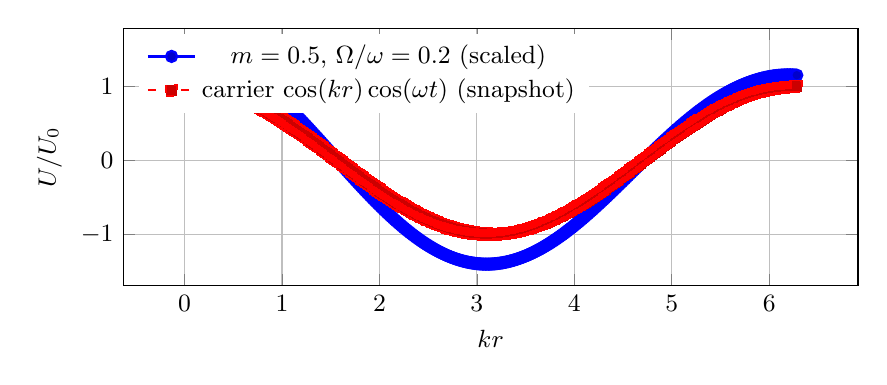
\begin{tikzpicture}
\begin{axis}[width=0.9\textwidth,height=0.4\textwidth,
    xlabel={$kr$}, ylabel={$U/U_0$}, grid=both, ticklabel style={font=\small}, label style={font=\small},
    legend style={font=\small, at={(0.02,0.98)}, anchor=north west, fill=white, draw=none}]
\addplot+[domain=0:6.283,samples=400,thick] {cos(deg(x))* (1 + 0.5*cos(deg(0.2*x)))};
\addlegendentry{$m=0.5$, $\Omega/\omega=0.2$ (scaled)}
\addplot+[domain=0:6.283,samples=400,thick,dashed] {cos(deg(x))};
\addlegendentry{carrier $\cos(kr)\cos(\omega t)$ (snapshot)}
\end{axis}
\end{tikzpicture}
\caption{Snapshot of a standing wave modulated in amplitude. The slow envelope (scaled representation of $\Omega\ll\omega$) multiplies the carrier.}
\label{fig:L1D}
\end{figure}

\subsection*{L.5.2 2D Interference of Two Modes (Energy Hot-Spot)}
\begin{figure}[h!]
\centering
\begin{tikzpicture}
\begin{axis}[width=0.9\textwidth,height=0.5\textwidth,
    xlabel={$kx$}, ylabel={$ky$}, view={0}{90},
    colormap/viridis, colorbar, point meta min=0, point meta max=2,
    ticklabel style={font=\small}, label style={font=\small}]
\addplot3[surf,shader=flat,domain=0:6.283,domain y=0:6.283,samples=101,samples y=101]
  {(cos(deg(x))+cos(deg(1.07*y)))^2};
\end{axis}
\end{tikzpicture}
\caption{Interference of two near-resonant standing patterns creates localized energy ``bubbles''. Squared field serves as a proxy for energy density.}
\label{fig:L2D}
\end{figure}

\subsection*{L.5.3 Time Map over One Modulation Period}
\begin{figure}[h!]
\centering
\begin{tikzpicture}
\begin{axis}[width=0.9\textwidth,height=0.45\textwidth,
    xlabel={$kr$}, ylabel={modulation phase $\Omega t / 2\pi$}, view={0}{90},
    colormap/viridis, colorbar,
    ticklabel style={font=\small}, label style={font=\small}]
\addplot3[surf,shader=flat,domain=0:6.283,domain y=0:1,samples=160,samples y=120]
  { (cos(deg(x)))^2 * (1 + 0.5*cos(deg(2*pi*y)))^2 };
\end{axis}
\end{tikzpicture}
\caption{Intensity map of a standing wave across one slow modulation period. High-intensity stripes at antinodes show how a slow envelope steers energy localization in time.}
\label{fig:Ltime}
\end{figure}

\section*{L.6 ISM Frequencies and Practical Targets}
Choosing ISM bands allows practical implementations: \SI{2.4}{GHz}, \SI{5}{GHz}, \SI{10}{GHz}.
Mode geometry (Appendix K) sets $k_\perp$; modulation $\Omega/2\pi$ in the \SI{}{\Hz}--\SI{}{\kilo\Hz} range suffices for slow coupling.
Targets: maximize antinode overlap with the $\psi$-sector projector by co-locating sensors at intensity hot-spots (Appendix I,E).

\section*{L.7 Compatibility with Existing Experiments}
Where $\psi=0$ (or averages to zero), UBT agrees with GR/Maxwell; no lab has reported curvature from EM standing waves at accessible powers, consistent with GR.
Therefore, any detected metric-sensitive effect in the above configurations bounds the UBT couplings.
Null results imply upper limits on $\|\Pi(\psi)\|$ and $\|\alpha_{\mu\nu}\|$; positive results indicate a $\psi$-mediated channel absent in GR.

\section*{L.8 Summary}
Standing and slowly modulated EM modes offer a curvature lever unique to UBT: by shaping $T^{\mu\nu}_{\rm EM,eff}$ and aligning it with the $\psi$-projector, one may obtain measurable metric perturbations without astronomical power.
This differs from GR while remaining compatible with all tests where $\psi$ vanishes or averages out.

\end{document}
